\documentclass[border=2mm]{standalone}
\usepackage{tikz}
\usetikzlibrary{shapes.geometric}

\begin{document}
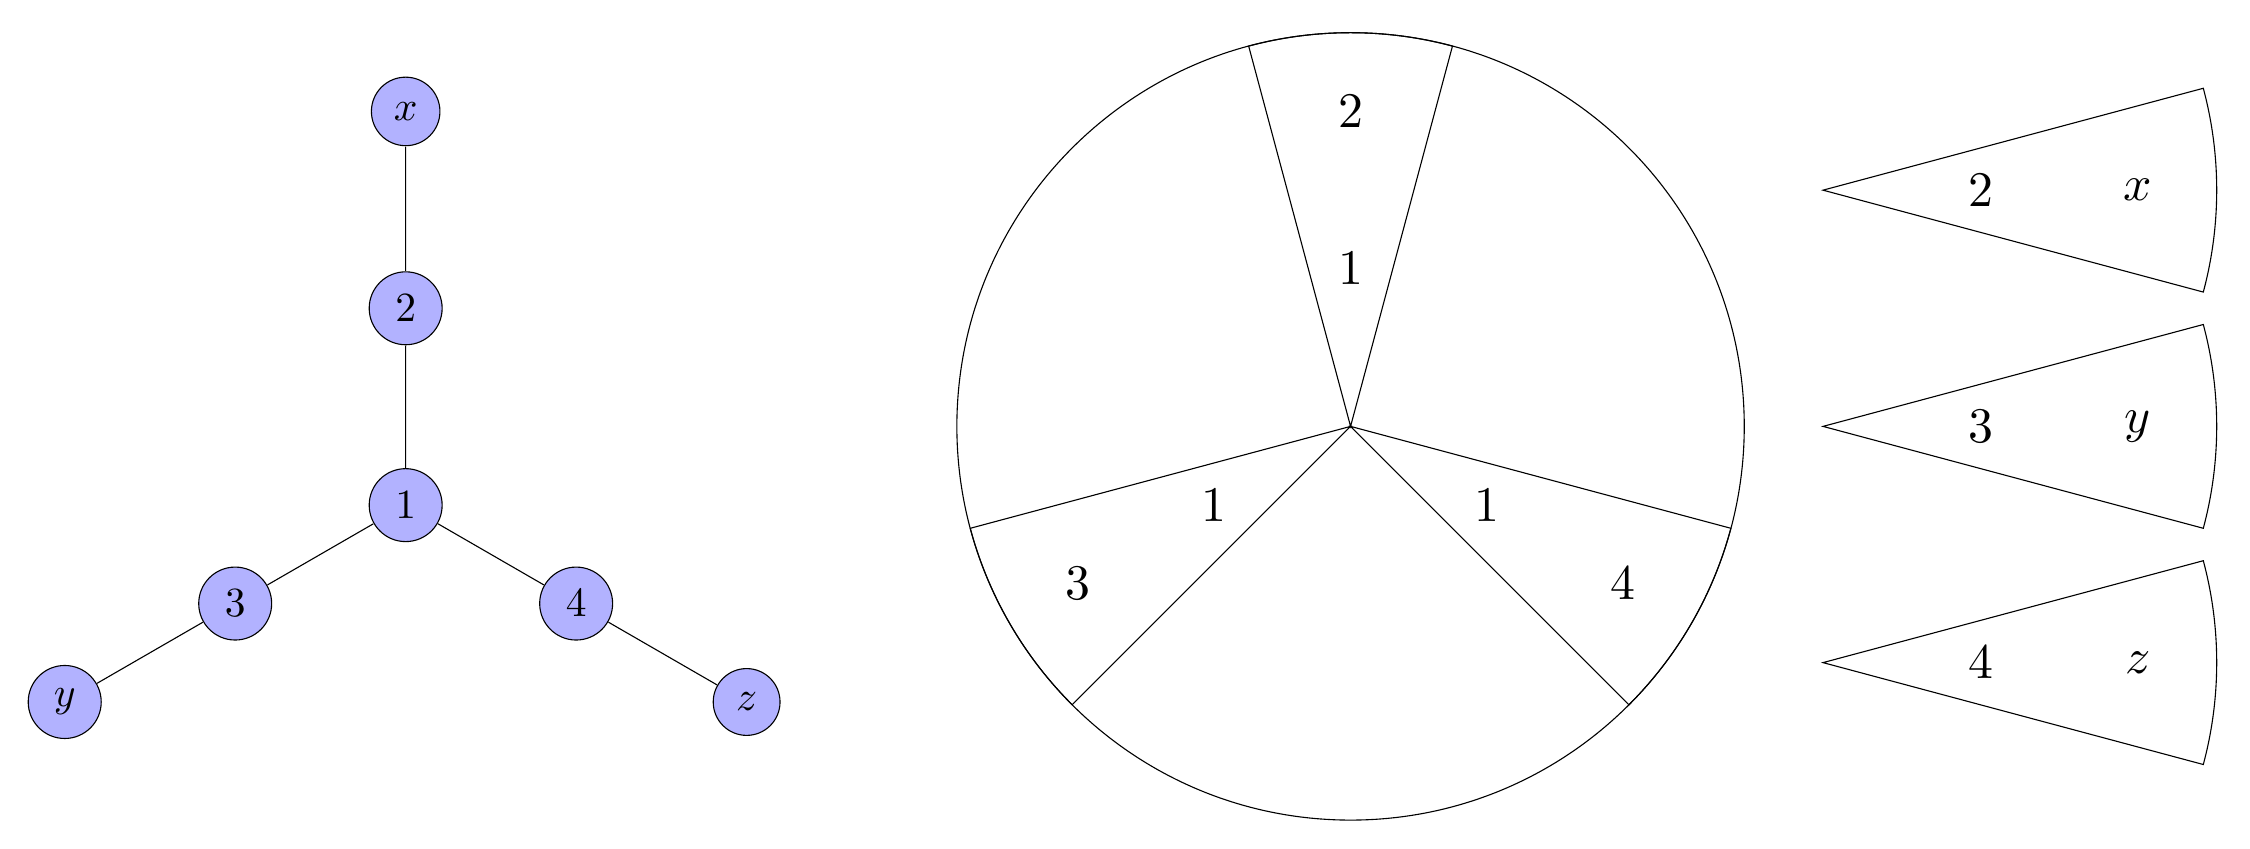
\begin{tikzpicture}[every node/.style={scale=1.8}]
  \draw (0,0) circle (5cm);
  \draw (0,0) -- (75:5) arc(75:105:5) -- cycle;
  \draw (0,0) -- (195:5) arc(195:225:5) -- cycle;
  \draw (0,0) -- (315:5) arc(315:345:5) -- cycle;
  \node at (90:2) {$1$};
  \node at (90:4) {$2$};
  \node at (210:2) {$1$};
  \node at (210:4) {$3$};
  \node at (330:2) {$1$};
  \node at (330:4) {$4$};
  \begin{scope}[shift={(6,3)}]
    \draw (0,0) -- (-15:5) arc(-15:15:5) -- cycle;
    \node at (0:2) {$2$};
    \node at (0:4) {$x$};
  \end{scope}
  \begin{scope}[shift={(6,0)}]
    \draw (0,0) -- (-15:5) arc(-15:15:5) -- cycle;
    \node at (0:2) {$3$};
    \node at (0:4) {$y$};
  \end{scope}
  \begin{scope}[shift={(6,-3)}]
    \draw (0,0) -- (-15:5) arc(-15:15:5) -- cycle;
    \node at (0:2) {$4$};
    \node at (0:4) {$z$};
  \end{scope}
  \begin{scope}[shift={(-12,-1)},every node/.style={draw,circle,scale=1.5,fill=blue!30}]
    \node (1) at (0,0) {$1$};
    \node (2) at (90:2.5) {$2$};
    \node (3) at (210:2.5) {$3$};
    \node (4) at (330:2.5) {$4$};
    \node (x) at (90:5) {$x$};
    \node (y) at (210:5) {$y$};
    \node (z) at (330:5) {$z$};
    \draw (1) -- (2) -- (x);
    \draw (1) -- (3) -- (y);
    \draw (1) -- (4) -- (z);
  \end{scope}
\end{tikzpicture}
\end{document}
